\documentclass[11pt,a4paper]{article}
\usepackage[latin1]{inputenc}
\usepackage{amsmath}
\usepackage{amsfonts}
\usepackage{amssymb}
\usepackage{array}
\usepackage{graphicx}
\usepackage{caption}
\usepackage{subcaption}
\author{Jordan Murray}
\title{EECS305 Lab4 Solutions}
\begin{document}
\begin{center}
\fontsize{24}{12}\selectfont
\textbf{Solution for Lab 4: System Type and Lead-Lag Control of a DC Servo Motor }
\end{center}

\section{Procedure}
\textbf{3.1 System Type and Tracking Error}

The Lab4\_SystemType.slx model contains five systems:
\begin{enumerate}
	\item step input, position feedback
	\item ramp input, position feedback
	\item parabolic input, position feedback
	\item step input, speed feedback
	\item ramp input, speed feedback
\end{enumerate}

The initial feedback gain for all five systems is 1.

For each system, we observe whether or not the reference is tracked, and if not, how the error evolves. We explore the effect of the feedback gain on the error signal.
\begin{enumerate}
	\item The step input is tracked with position feedback since the steady state error goes to zero.
	
	\begin{figure}[!htbp]
	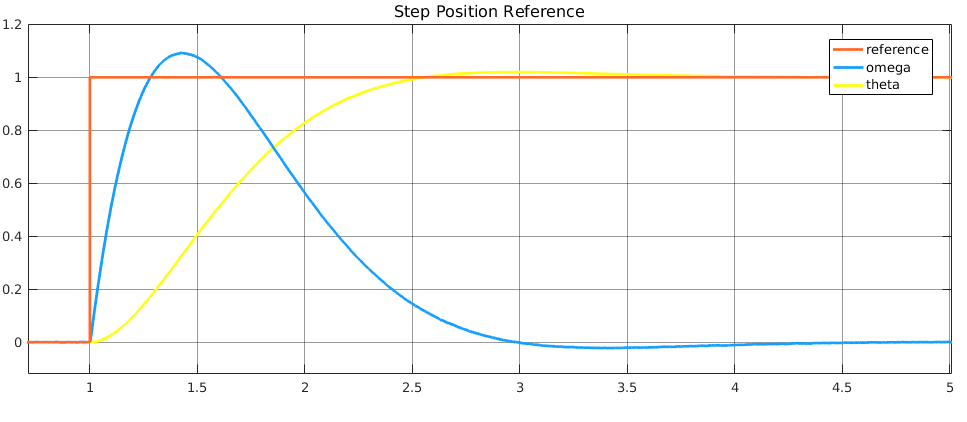
\includegraphics[width=\textwidth]{imglab/lab4sol_steppostraj.png}
	\caption{Position (yellow) tracks the reference (red).}
	\end{figure}
	
	\item The ramp input is not tracked with position feedback. The error approaches a constant value, implying that the speed implied by the slope of the reference is attained by the plant.

	\begin{figure}[!htbp]
	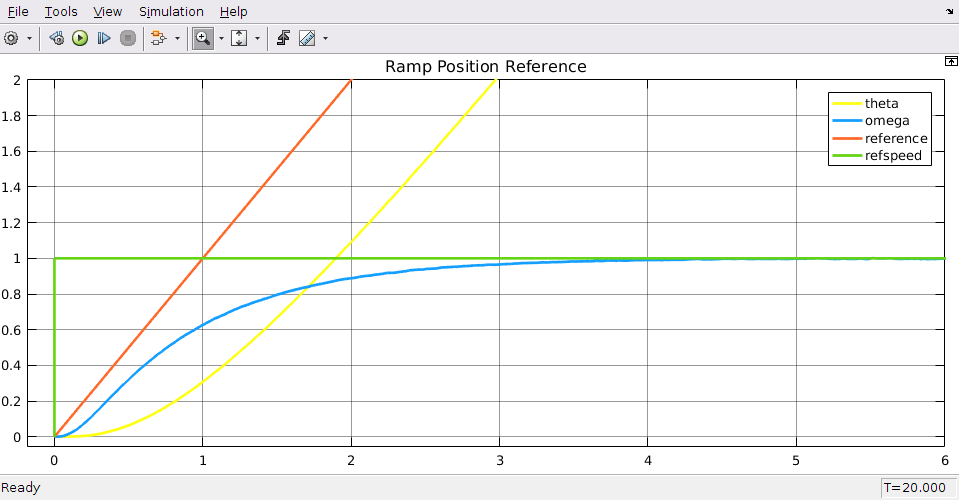
\includegraphics[width=\textwidth]{imglab/lab4sol_ramppostraj.png}
	\caption{Position(yellow) does not track the reference (red). However, the speed (blue) eventually matches the speed implied by the slope of the ramp (green). }
	\end{figure}	
	
	The effect of increasing the gain is illustrated by the following:
	
\begin{figure}[!htbp]
	\centering
	\begin{subfigure}{.5\textwidth}
		\centering
		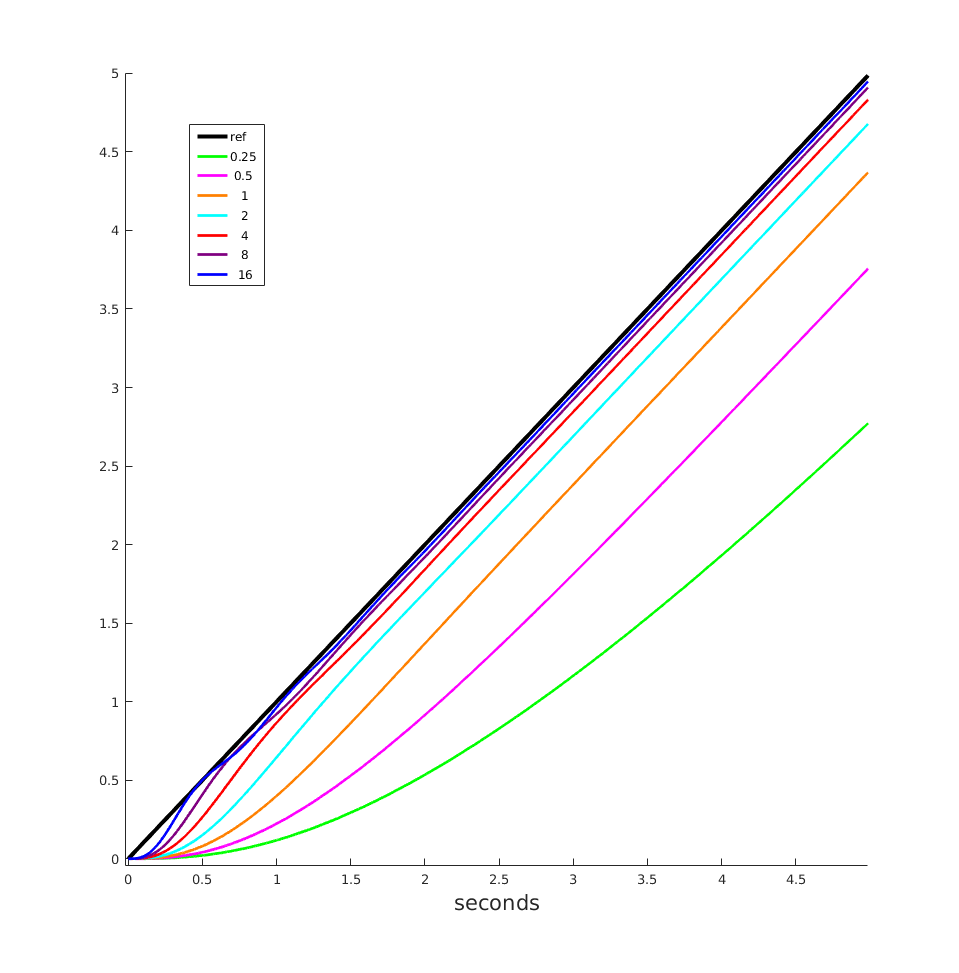
\includegraphics[width = \textwidth]{imglab/lab4sol_rampposkfam.png}
		\caption{Family of position trajectories for the following values of K: .25, .5, 1, 2, 4, 8.}
	\end{subfigure}%	
	\begin{subfigure}{.5\textwidth}
		\centering
		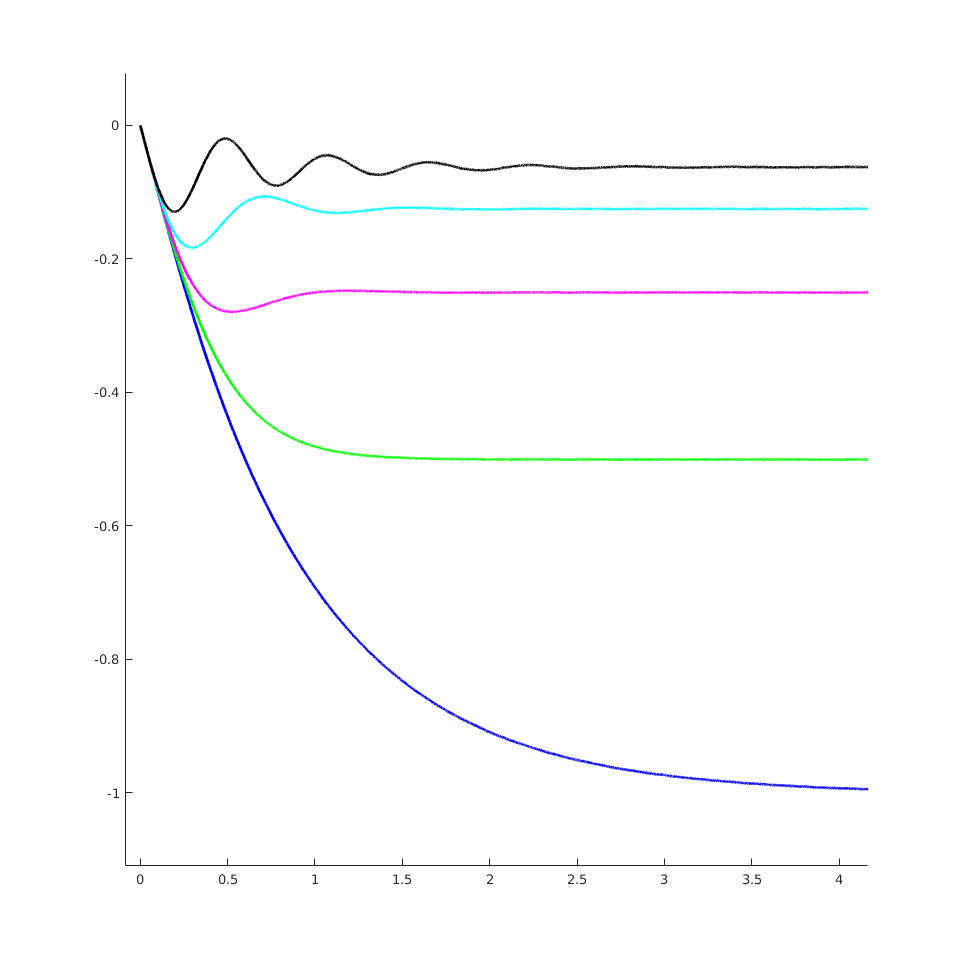
\includegraphics[width = \textwidth]{imglab/lab4sol_rampposerr.png}
		\caption{Family of position errors for the same K values.}	
	\end{subfigure}
\end{figure}
	
	Increasing the feedback gain reduces the limiting value of the position error, but does not completely eliminate it.
	
	\item The parabolic input is not tracked with position feedback. Position error increases linearly in time.
	
	\begin{figure}[!htbp]
	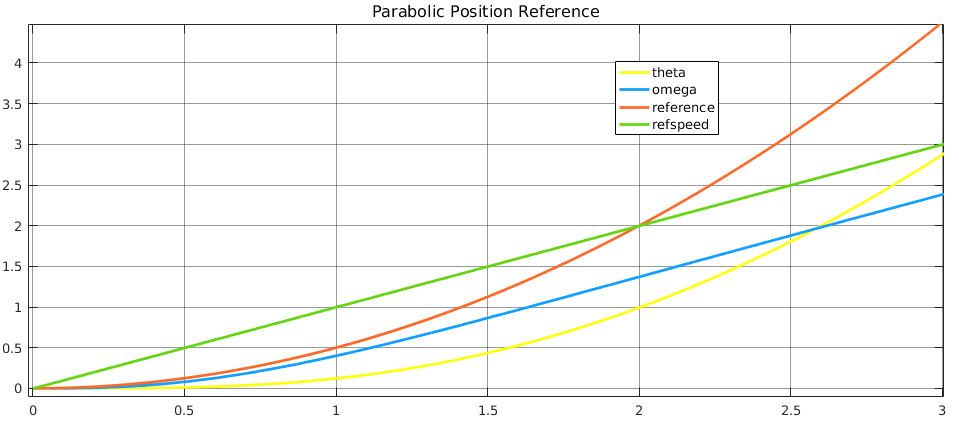
\includegraphics[width=\textwidth]{imglab/lab4sol_parapostraj.png}
	\caption{Position(yellow) does not track the reference (red). The speed implied by the derivative of the input eventually differs from the speed (blue) by a constant after}
	\end{figure}	
	
	The effect of increasing the gain is illustrated by the following:
	
\begin{figure}[!htbp]
	\centering
	\begin{subfigure}{.5\textwidth}
		\centering
		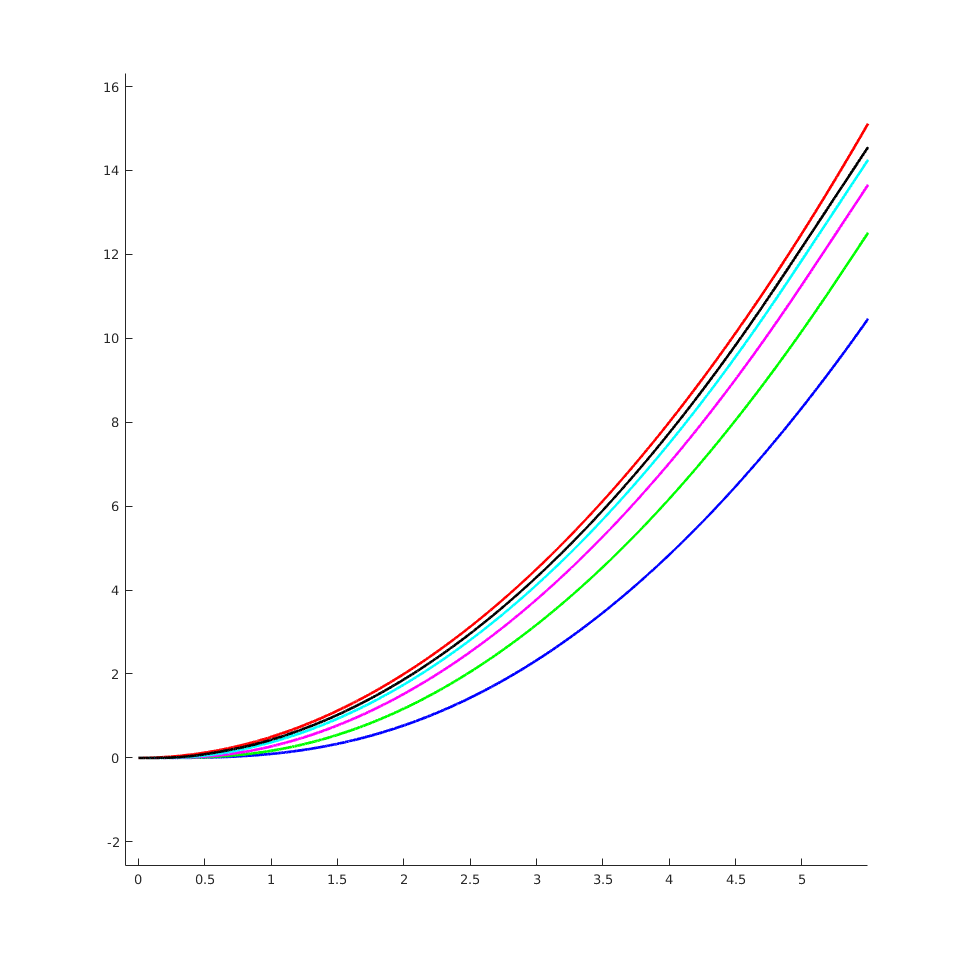
\includegraphics[width = \textwidth]{imglab/lab4sol_paraposkfam.png}
		\caption{A family of position curves for the same K values.}
	\end{subfigure}%	
	\begin{subfigure}{.5\textwidth}
		\centering
		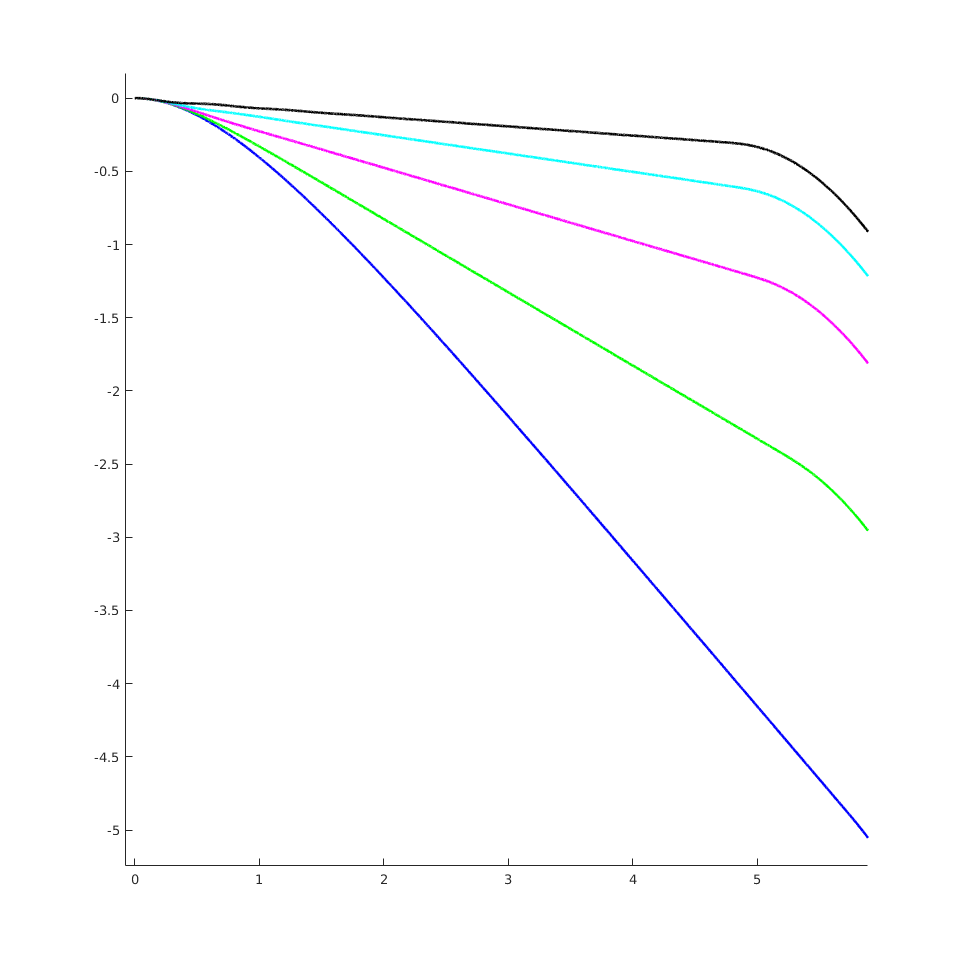
\includegraphics[width = \textwidth]{imglab/lab4sol_paraposerr.png}
		\caption{A family of position error curves for the same K values. The downturn at the right is due to the maximum speed of the servo being attained.}	
	\end{subfigure}
\end{figure}

Increasing the feedback gain can reduce the tracking error and decrease the constant rate at which the error increases, but it is not completely eliminated. 

	\item The step input is not tracked with speed feedback. The error approaches a constant value.
	
	\begin{figure}[!htbp]
	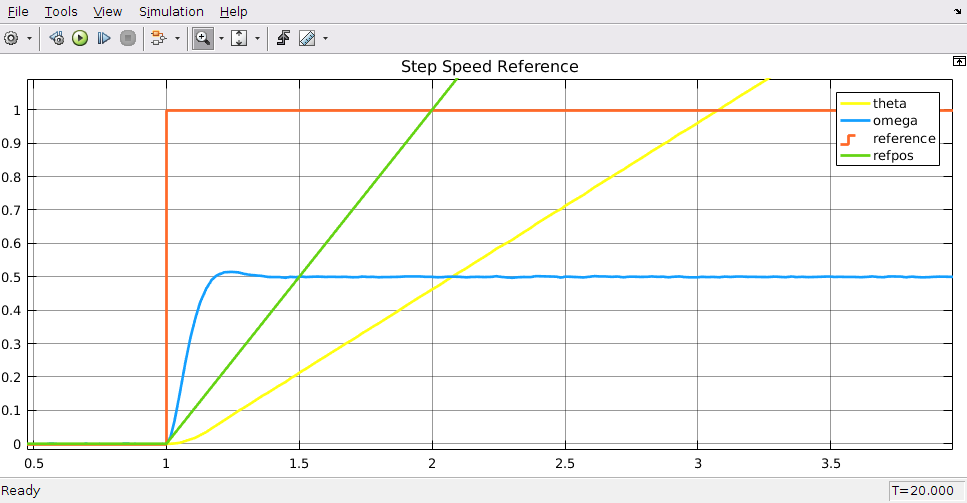
\includegraphics[width=\textwidth]{imglab/lab4sol_stepspeedtraj.png}
	\caption{Speed (blue) does not track the reference (red). The difference approaches a constant value.}
	\end{figure}	
	
		The effect of increasing the gain is illustrated by the following:
	
\begin{figure}[!htbp]
	\centering
	\begin{subfigure}{.5\textwidth}
		\centering
		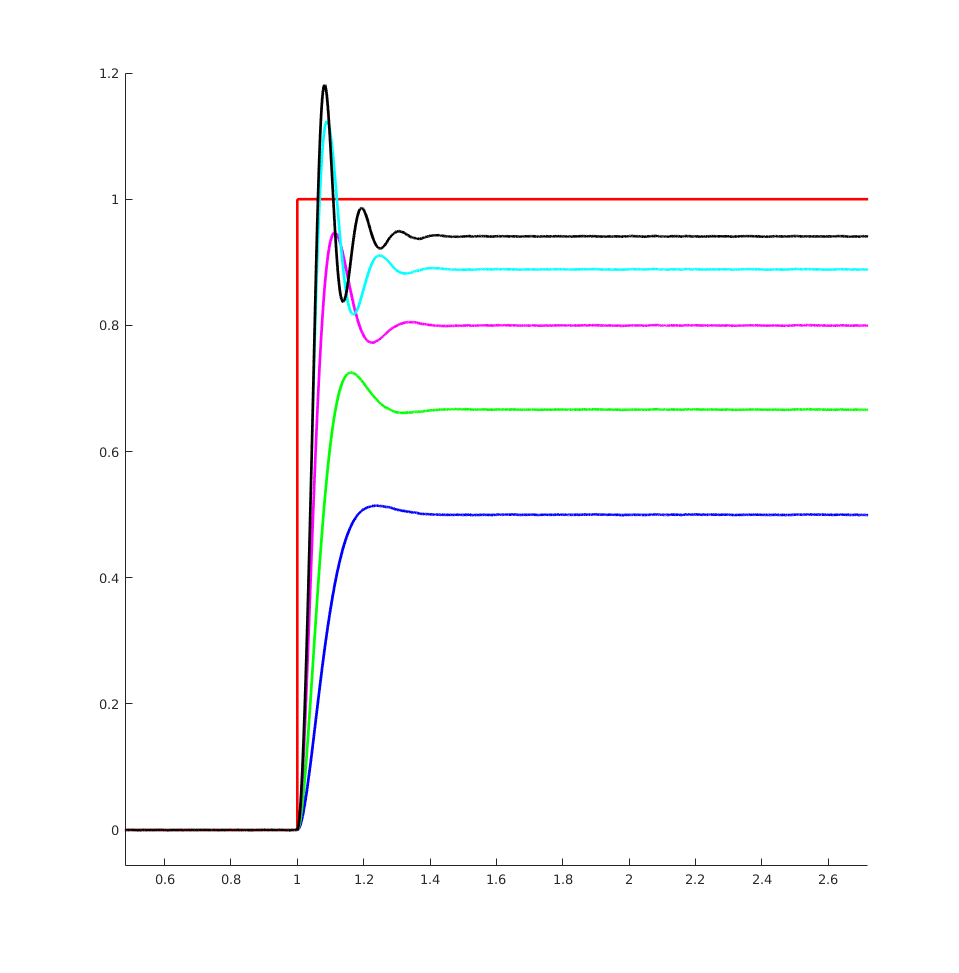
\includegraphics[width=\textwidth]{imglab/lab4sol_stepspeedkfam.png}
		\caption{Family of speed curves for the same values of K.}
	\end{subfigure}%	
	\begin{subfigure}{.5\textwidth}
		\centering
		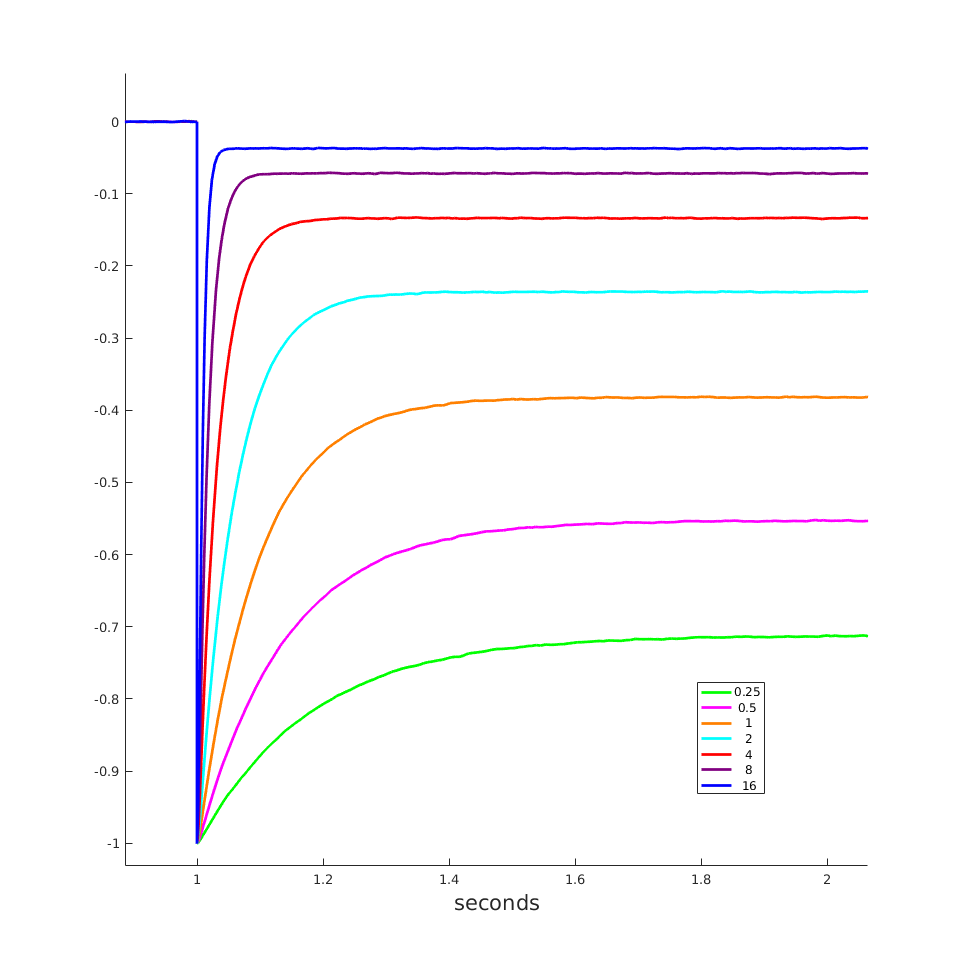
\includegraphics[width=\textwidth]{imglab/lab4sol_stepspeederr.png}
		\caption{Family of speed error curves for the same values of K. }	
	\end{subfigure}
\end{figure}

Increasing K reduces the steady state speed error, but does not eliminate it.
	
	\item The ramp input is not tracked with speed feedback. The error increases linearly in time.
	
	\begin{figure}[!htbp]
	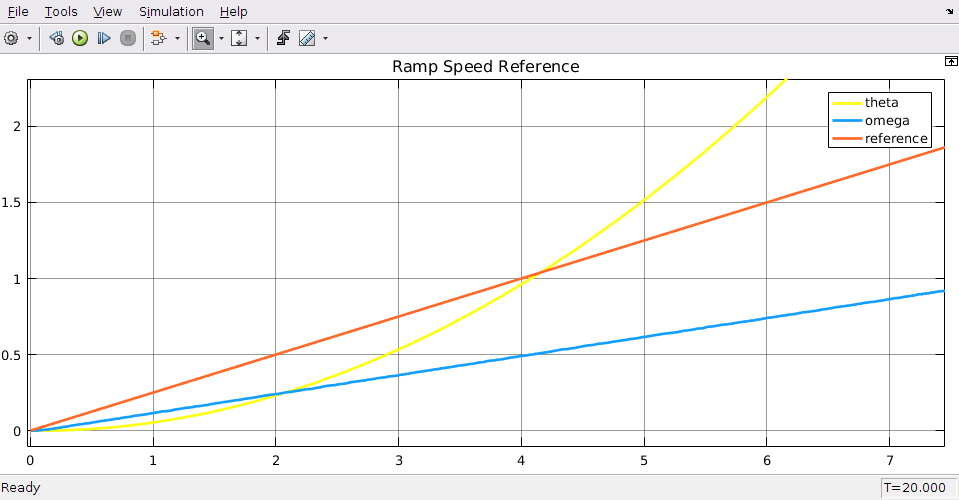
\includegraphics[width=\textwidth]{imglab/lab4sol_rampspeedtraj.png}
	\caption{The speed curve (blue) does not track the reference (red). The error increases linearly with time.}
	\end{figure}	
	
	The effect of increasing the gain is illustrated by the following:
	
\begin{figure}[!htbp]
	\centering
	\begin{subfigure}{.5\textwidth}
		\centering
		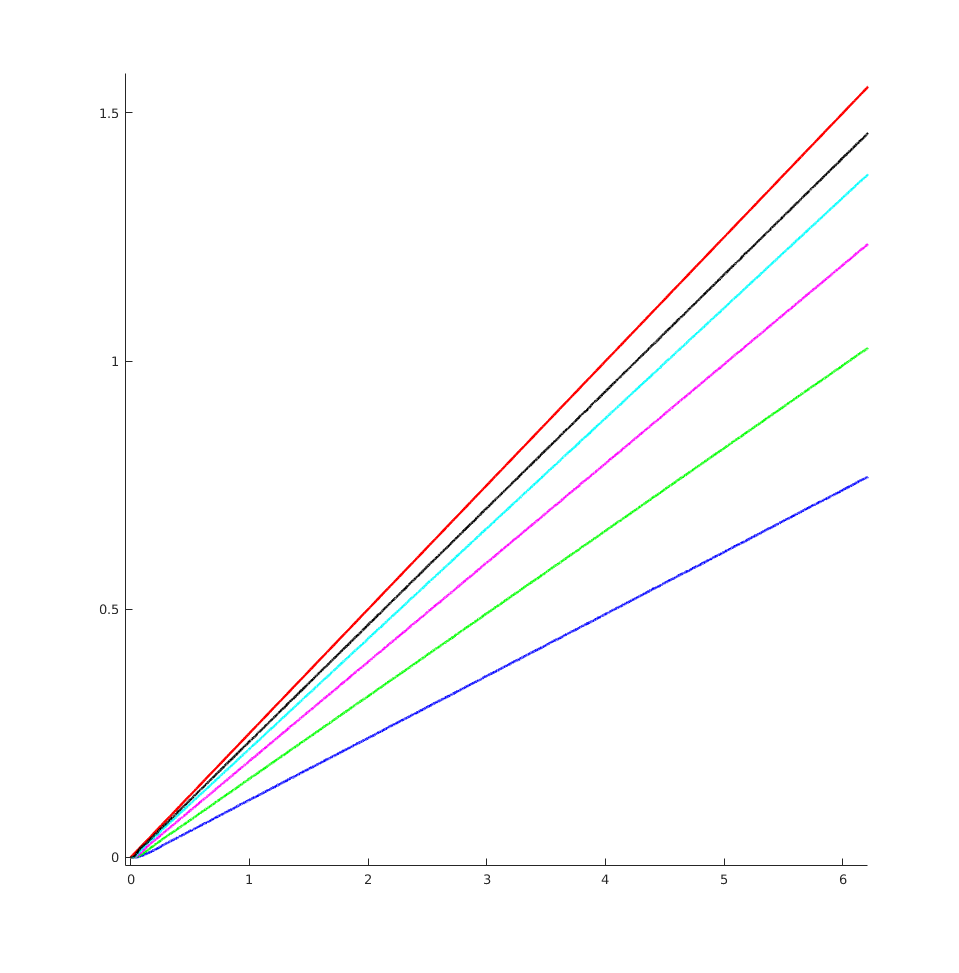
\includegraphics[width = \textwidth]{imglab/lab4sol_rampspeedkfam.png}
		\caption{A family of speed curves for the same values of K.}
	\end{subfigure}%	
	\begin{subfigure}{.5\textwidth}
		\centering
		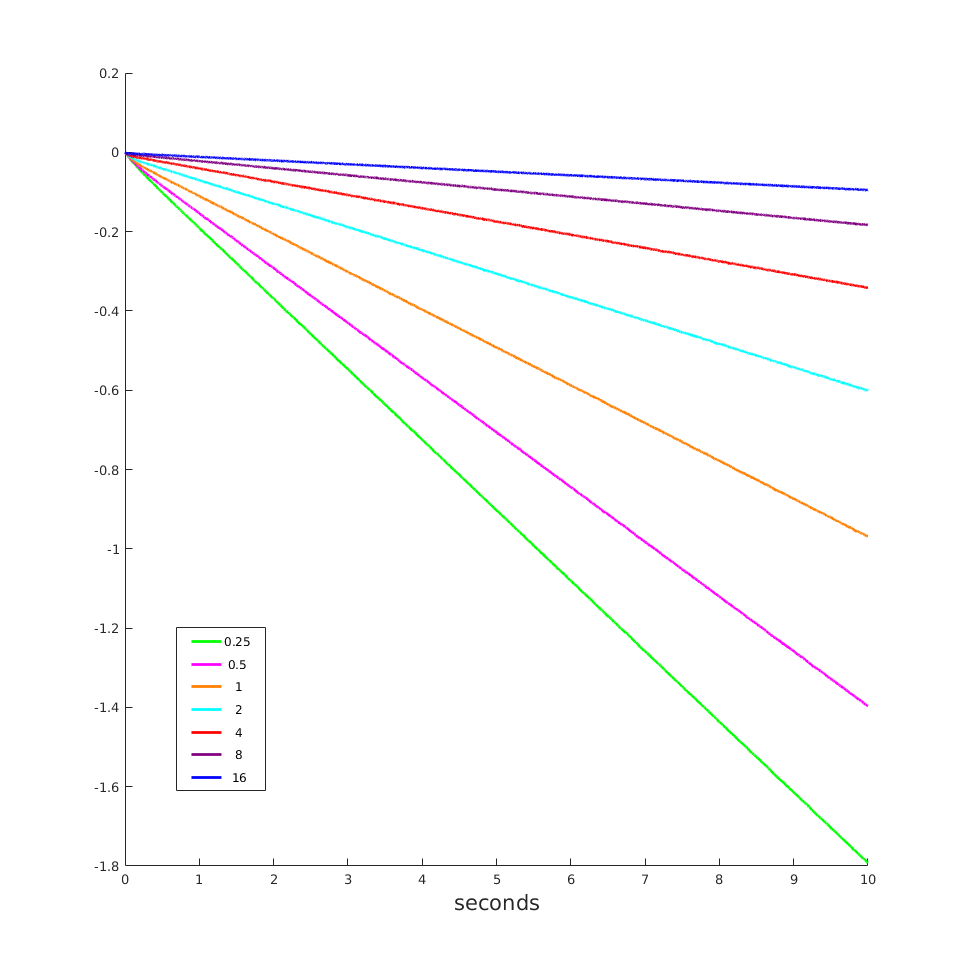
\includegraphics[width = \textwidth]{imglab/lab4sol_rampspeederr.png}
		\caption{A family of speed error curves for the same values of K.}	
	\end{subfigure}
\end{figure}

Increasing the feedback gain reduces the steady state error and the rate at which it increases, but does not completely eliminate it.
	
\end{enumerate}

\textbf{3.2 Identify $K_{s}$ and $\tau$}

\begin{figure}[!htbp]
	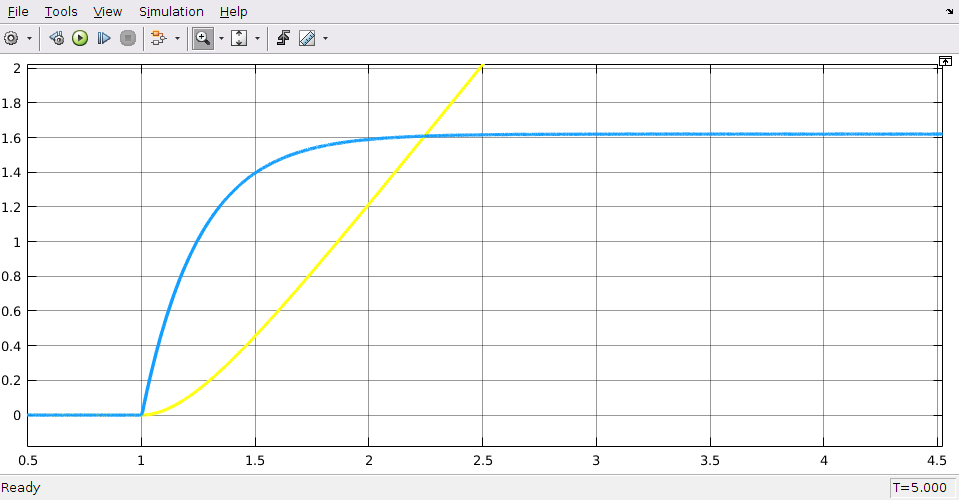
\includegraphics[width=\textwidth]{imglab/lab4sol_identification.png}
	\caption{Speed trajectory (blue) for a unit step input.}
\end{figure}

We run the Simulink model Lab4\_Identification.slx which applies a unit step to the open loop system at t=1 and estimate steady state value of the speed to be 1.62, implying a $K_{s}$ of 1.62. We then estimate the time at which the output reaches 63.2\% of its steady state value, or 1.0238, to be 1.254, implying a $\tau$ of .254.


\textbf{3.3 Proportional Feedback}

	The Simulink model Lab4\_ProportionalFeedback.slx contains a DC servo model with proportional feedback fed with a unit step input at t=1. We minimize the system's settling time subject to a 5\% limit on maximum overshoot. 	
	
	We use Matlab's rlocus() function to plot our DC servo transfer function's root locus. The function sgrid($\zeta$,$\omega_{n}$) with a $\zeta$ of .6901 plots the boundary of the region in the s plane that our closed loop poles may occupy. The function rlocfind() is then used to find a range of feedback gains corresponding to points on the root locus between the divergence from the real axis and the damping ratio boundary. Feedback gains over this region range roughly from .6 to 1.2. A gain of .9 results in a settling time of about 1.65s with an overshoot of about 1\%.


\begin{figure}[!htbp]
	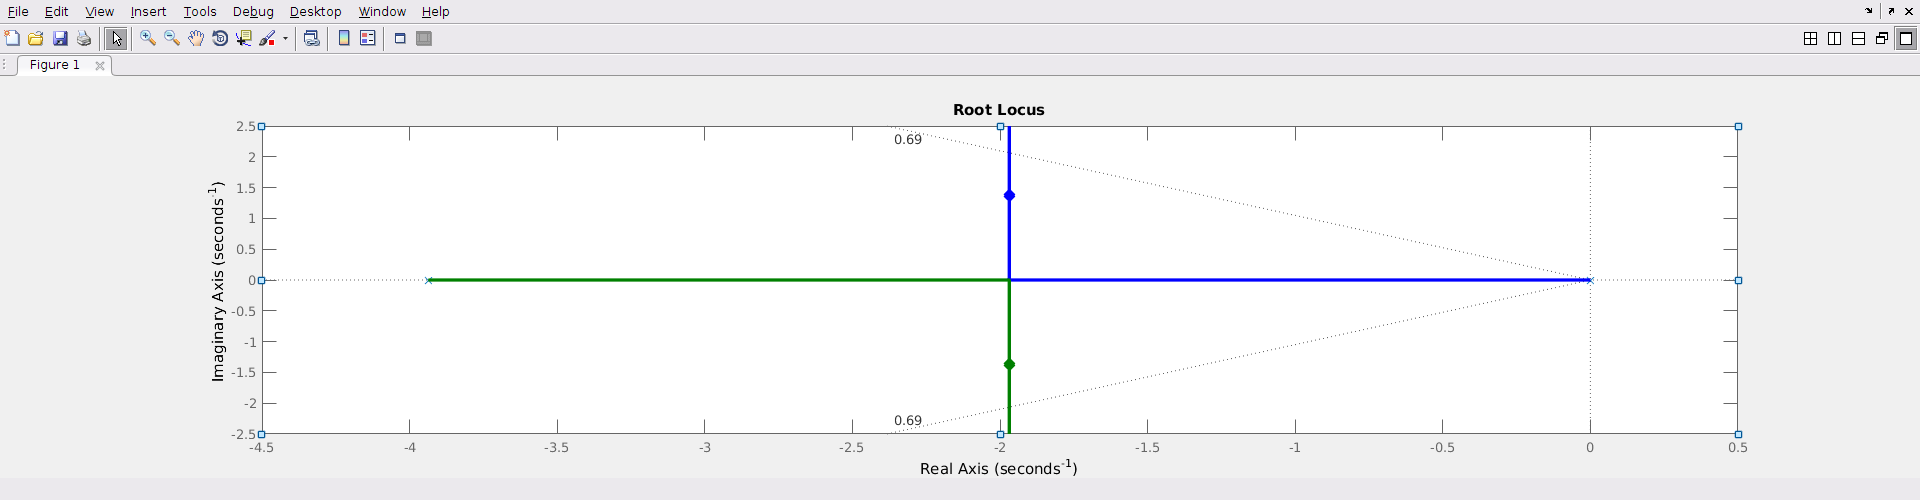
\includegraphics[width=\textwidth]{imglab/lab4sol_constantrloc.png}
	\caption{The DC servo system's root locus. The markers indicate the pole locations corresponding to a gain of .9.}
\end{figure}



\begin{figure}[!htbp]
	\centering
	\begin{subfigure}{.5\textwidth}
		\centering
		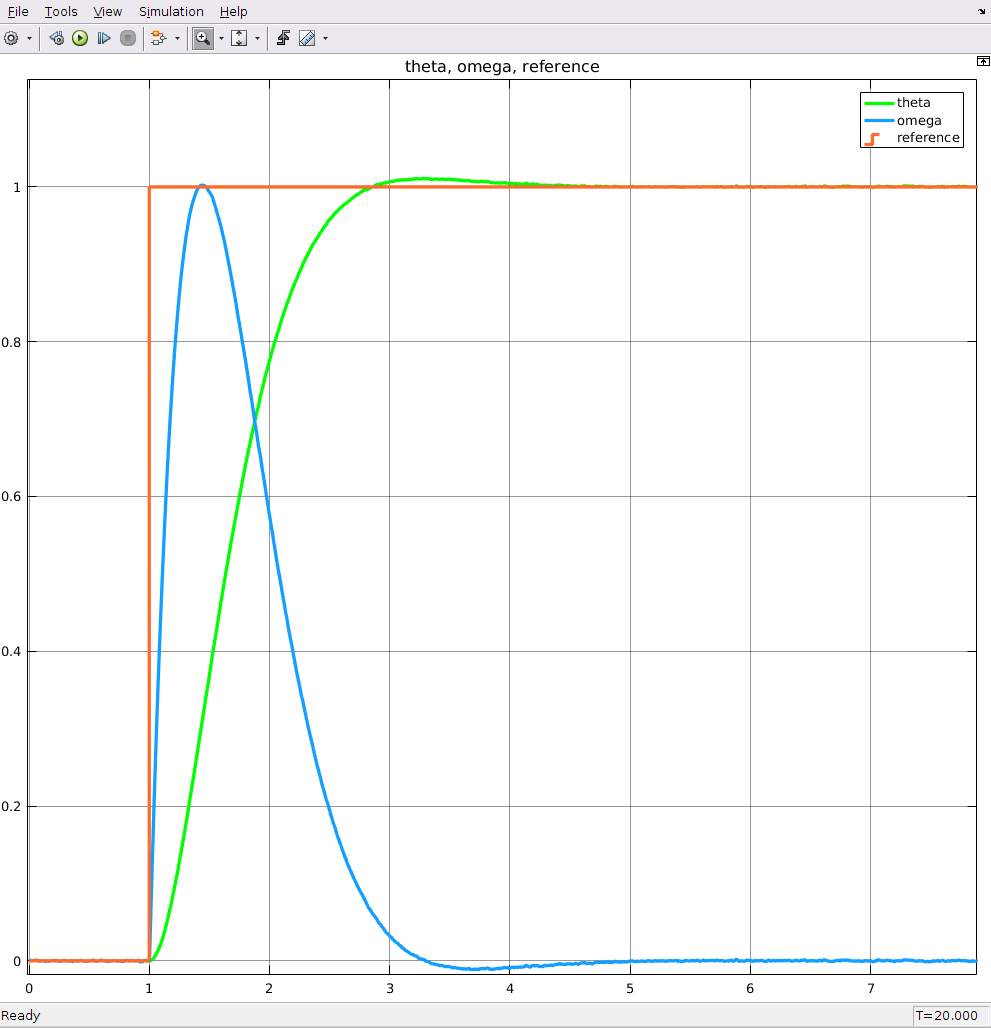
\includegraphics[width = \textwidth]{imglab/lab4sol_constanttraj.png}
		\caption{Position trajectory for proportional with K = .9.}
	\end{subfigure}%	
	\begin{subfigure}{.5\textwidth}
		\centering
		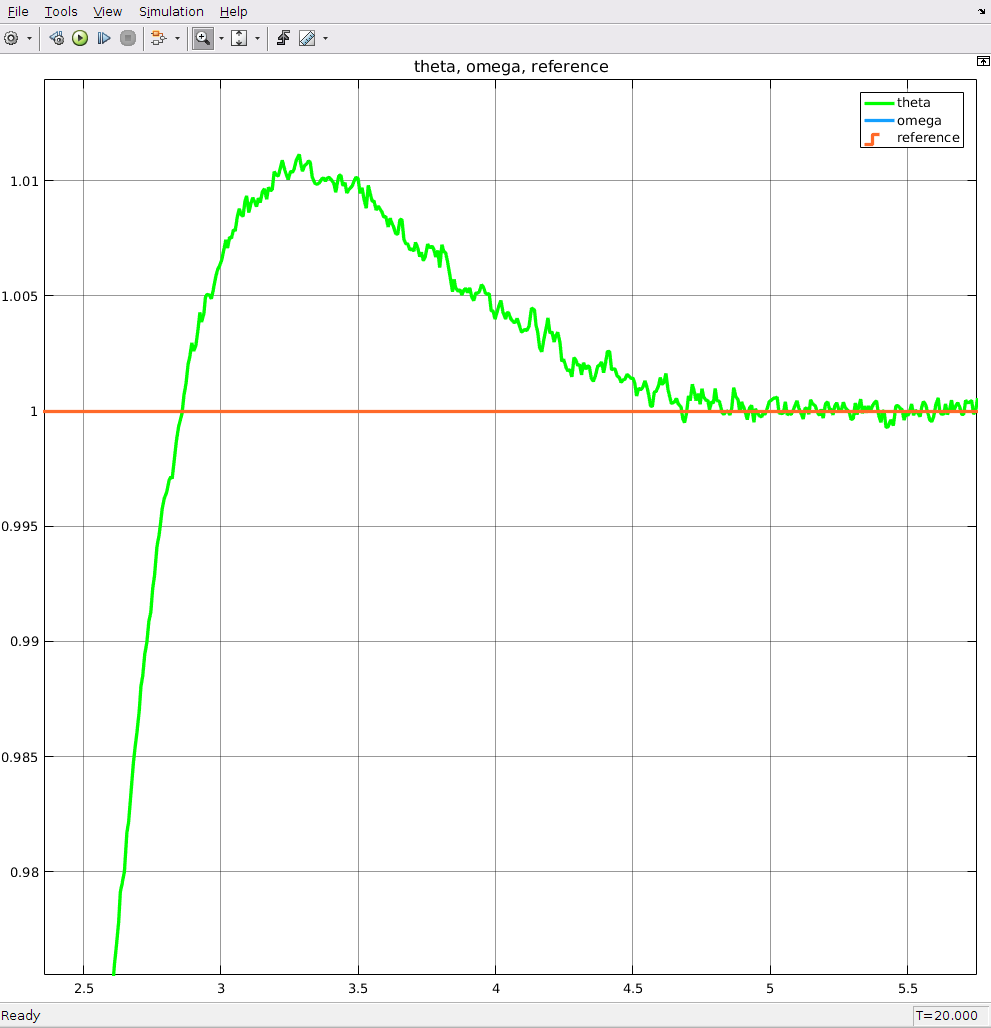
\includegraphics[width = \textwidth]{imglab/lab4sol_constanttrajclose.png}
		\caption{Closeup view of peak of the same.}	
	\end{subfigure}
\end{figure}



\textbf{3.4 Lead Compensation}

The specifications for our controller are:
\begin{enumerate}
\item Overshoot less than 5\%.
\item 2\% band settling time less than .6 seconds
\end{enumerate}

We first determine the damping ratio $\zeta$ and natural frequency $\omega_{n}$ corresponding to these constraints.

From the formula for maximum overshoot we have:
\begin{equation}
	\zeta = \sqrt{\frac{\ln (M)^{2}}{\pi^{2} + \ln (M)^{2}}}
\end{equation}
where M is the maximum overshoot (.05).

From the formula for the envelope of the oscillations, we have:
\begin{equation}
	\omega_{n} = \frac{1}{\zeta t_{s}} \log \left( \frac{1}{\epsilon \sqrt{1 - \zeta^{2}}} \right)
\end{equation}
alternatively, we could use the less precise formula:
\begin{equation}
	\omega_{n} = \frac{4}{\zeta t_{s}}
\end{equation}
where $t_{s}$ is the settling time for the 2\% band (.6).

We will use the first formula for the natural frequency, yielding $\omega_{n} = 10.2288$ and $\zeta = .6901$. We now determine the desired location of our dominant closed loop poles according to the formula: 

\begin{equation}
	s = \sigma + j \omega = \zeta \omega_{n} + j \omega_{n} \sqrt{1 - \zeta^{2}}
\end{equation}

which yields pole locations of $ -7.0590 \pm j 7.4027$. 

Now we will determine the position of the lead controller pole and zero such that the desired closed loop pole locations are on the root locus. The angle condition tells us that

\begin{equation}
	\angle G(s)H(s) = \pi
\end{equation}

which implies

\begin{equation}
	\angle z_{lead} - \angle p_{lead}   =  \pi + \angle p_{ol1} + \angle p_{ol2}
\end{equation}

indicating that the difference between the lead pole angle and zero angle must be 1.1607 radians. In the limit that the lead compensator pole is at $-\infty$, its angle will be zero and the the lead zero angle must be 1.1607, corresponding to -10.2769 on the real axis. This is the farthest left we can place the zero.

 We choose to place the zero at -8.668, at an angle of 1.3568 radians, leaving .1960 radians for the lead controller pole angle. This corresponds to a pole location of -44.3358.

We now use the gain condition to find the appropriate gain for our lead controller. 
\begin{equation}
	K \frac{\lvert s + z_{1} \rvert \lvert s + z_{2} \rvert \cdots \lvert s + z_{m} \rvert }{\lvert s + p_{1} \rvert \lvert s + p_{2} \rvert \cdots \lvert s + p_{n} \rvert} = 1
\end{equation}

In our case,

\begin{equation}
	K \frac{\lvert \frac{1.62}{.254} \rvert \lvert s + 8.668 \rvert}{ \lvert s + 44.3358 \rvert \lvert s + 0 \rvert  \lvert s + 3.9370 \rvert} = 1
\end{equation}
 
 substituting our desired pole location for s and solving for K,  we get 64.6407. 
 
 
\begin{figure}[!htbp]
	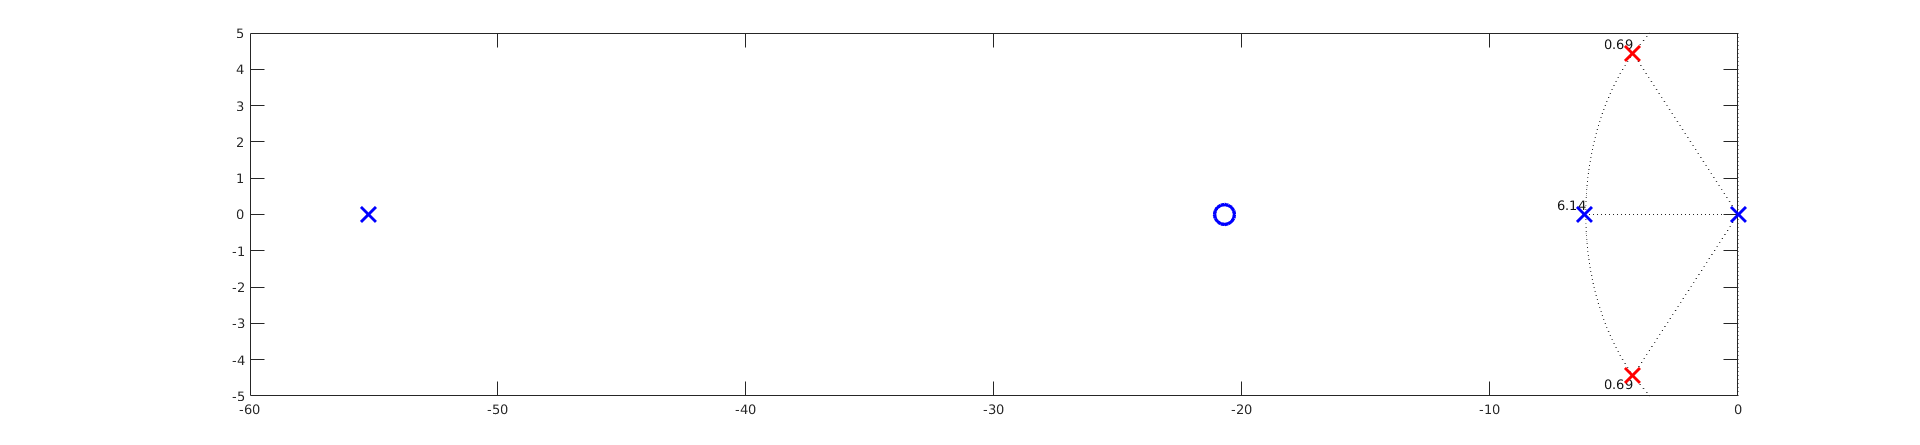
\includegraphics[width=\textwidth]{imglab/lab4sol_leadpoles.png}
	\caption{ The root locus with open loop poles and zeros in blue and the dominant closed loop poles in red on the s plane with damping ratio and natural frequency constraints.}
\end{figure}



We use the Simulink model Lab4\_Lead.slx to demonstrate the controller's performance. Two systems receive a unit step input as a position reference. Factoring out the zero and pole from lead compensator transfer function so that it will have unity steady state gain gives us a compensator transfer function
\begin{equation}
	\frac{.1154s + 1}{.02256s + 1}
\end{equation}

and a gain of 12.6377. For the system with the compensator in the feedback path, we have a peak overshoot of 5.0\% and a settling time of .59 seconds, which meets our requirements. For the system with the compensator in the forward path, the maximum overshoot is 15.7\% and the settling time is .51 seconds.

\begin{figure}[!htbp]
	\centering
	\begin{subfigure}{.5\textwidth}
		\centering
		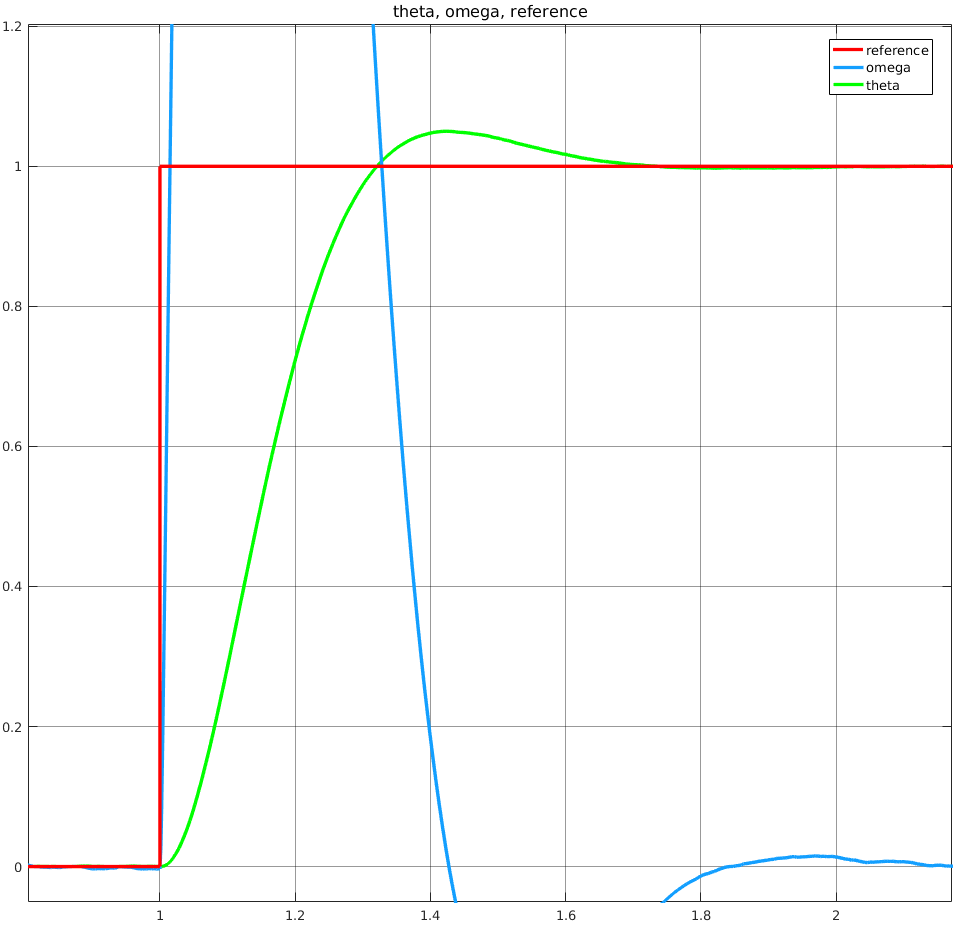
\includegraphics[width = \textwidth]{imglab/lab4sol_leadtrajfeedback.png}
		\caption{Position vs. time with lead controller in feedback path.}
	\end{subfigure}%	
	\begin{subfigure}{.5\textwidth}
		\centering
		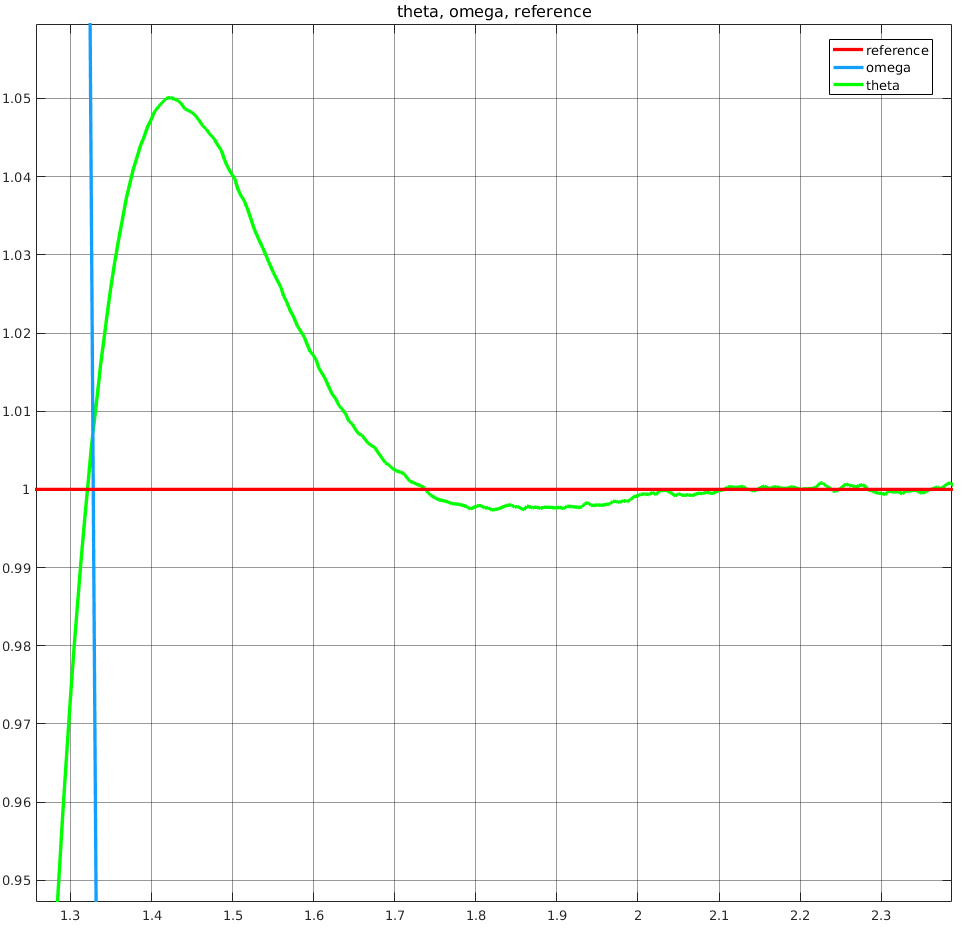
\includegraphics[width = \textwidth]{imglab/lab4sol_leadtrajfeedbackclose.png}
		\caption{Close up of position trajectory.}	
	\end{subfigure}
\end{figure}

\begin{figure}[!htbp]
	\centering
	\begin{subfigure}{.5\textwidth}
		\centering
		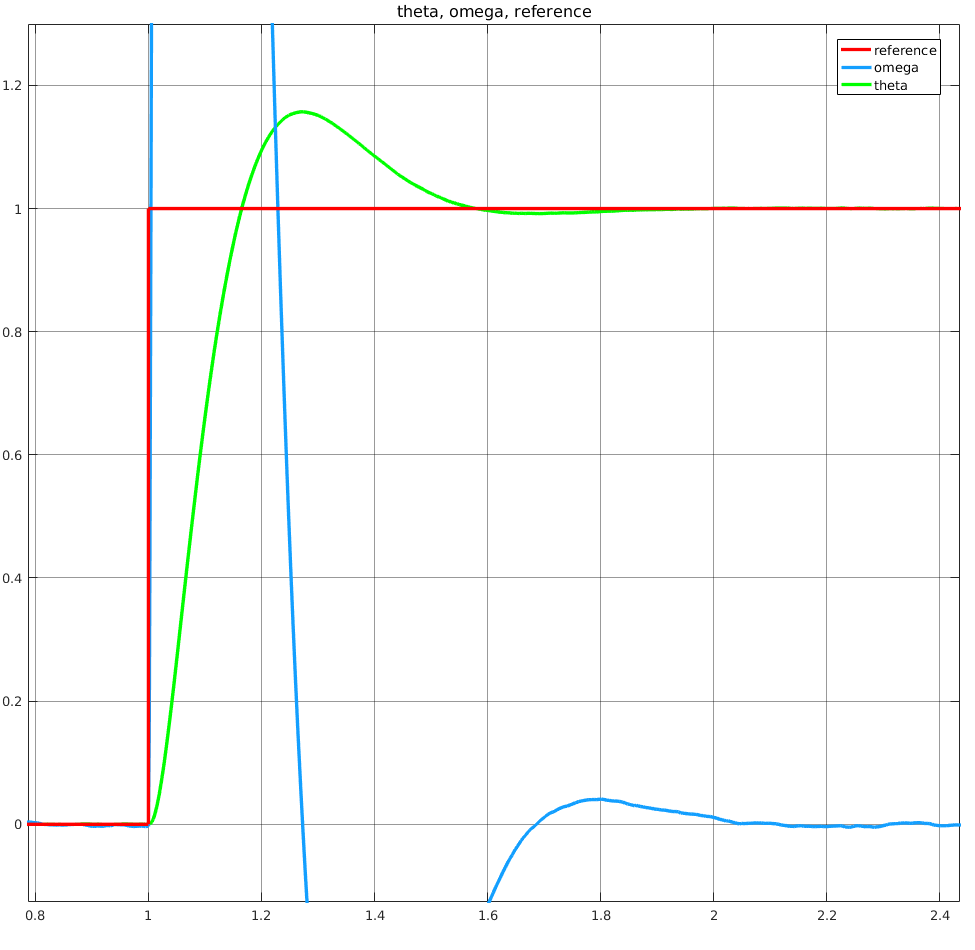
\includegraphics[width = \textwidth]{imglab/lab4sol_leadtrajforward.png}
		\caption{Position vs. time with lead controller in forward path.}
	\end{subfigure}%	
	\begin{subfigure}{.5\textwidth}
		\centering
		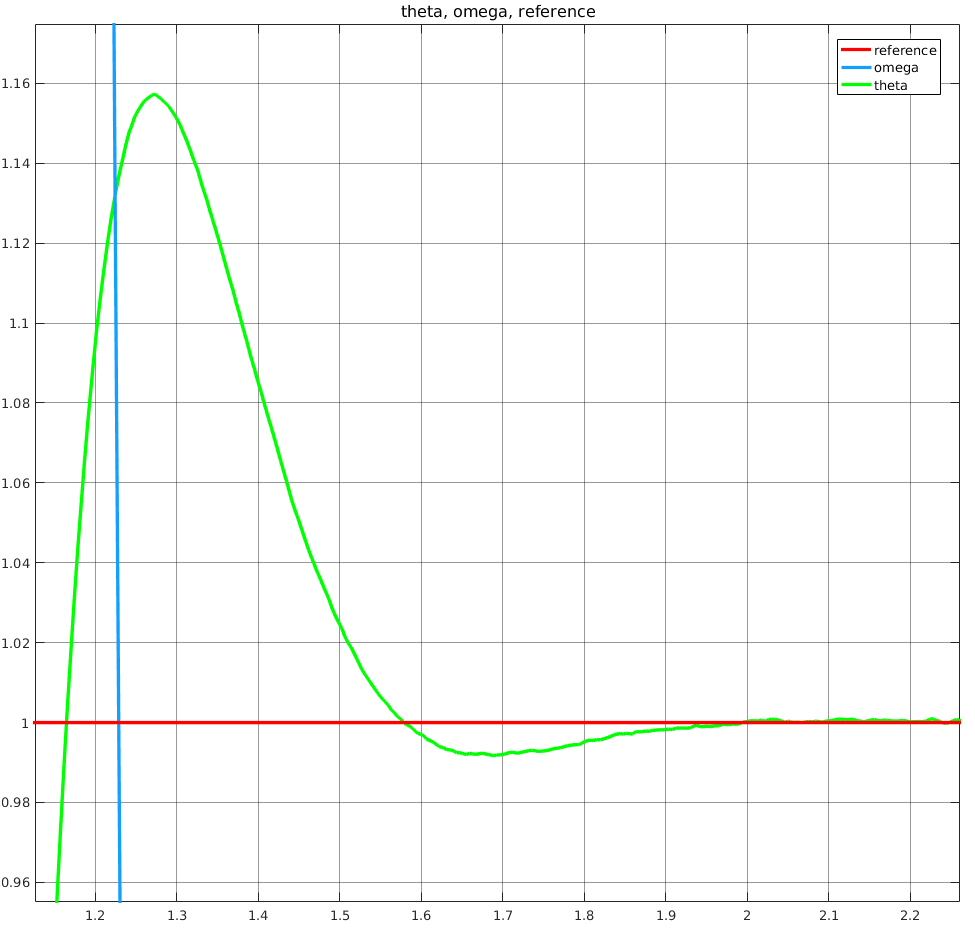
\includegraphics[width = \textwidth]{imglab/lab4sol_leadtrajforwardclose.png}
		\caption{Close up of position trajectory.}	
	\end{subfigure}
\end{figure}

The difference in performance can be understood by considering the difference in the closed loop zeros. Let the open loop servo transfer function G(s) be $\frac{N_{servo}(s)}{D_{servo}(s)}$ and the lead compensator transfer function H(s) be $\frac{N_{lead}(s)}{D_{lead}(s)}$ Where N is numerator and D is the denominator of the transfer functions. The closed loop transfer function for the system with the compensator in the feedback is
\begin{equation}
	\frac{KG(s)}{1+KG(s)H(s)}
\end{equation}
or, in terms of the N(s) and D(s):
\begin{equation}
	\frac{K N_{servo}(s) D_{lead}(s)}{D_{servo}(s) D_{lead}(s) + K N_{servo} N_{lead}}
\end{equation}

and the transfer function for the system with the compensator in the forward path is
\begin{equation}
	\frac{KG(s)H(s)}{1+KG(s)H(s)}
\end{equation}
or, in terms of the N(s) and D(s):
\begin{equation}
	\frac{K N_{servo}(s) N_{lead}(s)}{D_{servo}(s) D_{lead}(s) + K N_{servo} N_{lead}}
\end{equation}

Though we have positioned the poles that we hope will be dominant through our lead compensator design, the remaining pole will also contribute to the response. Though the poles are the same for both configurations, the magnitude of each component of the response will depend on the zeros.

\textbf{3.5 Lead-Lag Compensation}


\section{Exercises}

\begin{enumerate}
\item \textbf{System Type and Tracking Error}
From the final value theorem we know:
\begin{equation}
	\lim_{t \to \infty} f(t) = \lim_{s \to 0}sF(s)
\end{equation}

or more specifically, in our case:
\begin{equation}
	\lim_{t \to \infty} f(t) = \lim_{s \to 0}sU(s)G^{\prime}(s)
\end{equation}

where $G^{\prime}(s)$ is the closed loop transfer function for G(s), the input to position transfer function for the servo system.

For a position feedback system with a step input, we have:

\begin{equation}
	\lim_{t \to \infty} f(t) = \lim_{s \to 0}s\frac{R}{s}\frac{K_{s}K_{1}}{\tau s^{2} + s + K_{1}K_{s}} = R
\end{equation}

therefore, the steady-state value is equal to the reference value.

For a position feedback system with a ramp input, we have:
\begin{equation}
	\lim_{t \to \infty} f(t) = \lim_{s \to 0}s\frac{1}{s^{2}}\frac{K_{s}K_{1}}{\tau s^{2} + s + K_{1}K_{s}} = \infty
\end{equation}

As expected, the position trajectory has no steady state value.

Using the Final Value Theorem we can find the steady state error:
\begin{equation}
	\lim_{t \to \infty} e(t) 
	= \lim_{s \to 0}s\frac{1}{s^{2}}(1 - \frac{K_{s}K_{1}}{\tau s^{2} + s + K_{1}K_{s}})
\end{equation}
\begin{equation}	
	 = \lim_{s \to 0}\frac{1}{s}\frac{\tau s^{2} + s}{\tau s^{2} + s + K_{1}K_{s}} 
\end{equation}
\begin{equation}	
	= \lim_{s \to 0}\frac{\tau s^{2} + s}{\tau s^{3} + s^{2} + K_{1}K_{s}s} 
\end{equation}

\begin{equation}
	= \frac{1}{K_{1}K_{s}}
\end{equation}

which confirms our suspicion that there is no value of $K_{1}$ which will completely eliminate the steady-state error.

For a position feedback system with a parabolic input, we can see from the foregoing that the limit of the error will be infinity:

\begin{equation}
	\lim_{t \to \infty} e(t) 
	= \lim_{s \to 0}s\frac{1}{s^{3}}(1 - \frac{K_{s}K_{1}}{\tau s^{2} + s + K_{1}K_{s}})
\end{equation}
with the extra s in the denominator, we end up with:

\begin{equation}
	\lim_{s \to 0}\frac{1}{2K_{1}K_{s}s + O(s^{2})} = \infty
\end{equation}


However, if we look instead at the final value of the derivative of the error, we cancel this extra s and show that the derivative of the error has a constant value, or that the error increases linearly in time.

For speed feedback systems, we must use the input to speed transfer function instead.

For a speed feedback system with a step reference, we have the final value:
\begin{equation}
	\lim_{t \to \infty} f(t) = \lim_{s \to 0}s\frac{R}{s}\frac{K_{s}K_{1}}{\tau s + s + K_{1}K_{s} + 1} = R \frac{K_{s}K_{1}}{K_{s}K_{1}+1}
\end{equation}
and a steady state error of

\begin{equation}
	\frac{R}{K_{s}K_{1} + 1}
\end{equation}

For a speed feedback system with a ramp reference, we have an additional s in the denominator, making the error infinite

\begin{equation}
	\lim_{t \to \infty} e(t) 
	= \lim_{s \to 0}s\frac{1}{s^{2}}(1 - \frac{K_{s}K_{1}}{\tau s^ +  K_{1}K_{s} + 1})
\end{equation}

\begin{equation}
	= \lim_{s \to 0}\frac{1}{s}\frac{\tau s + 1}{\tau s +  K_{1}K_{s} + 1} = \infty
\end{equation}

However, we can again cancel this extra s by considering the derivative of the error, showing that the error also increases linearly in this case. 

Writing an open loop transfer function G(s) as $\frac{N(s)}{D(s)}$, we can see that for the closed loop transfer function $G^{\prime}(s) = \frac{K_{1}G(s)}{1+K_{1}G(s)}$ we will have 
\begin{equation}
	\frac{K_{1}N(s)}{D(s) + K_{1}N(s)}
\end{equation}

In calculating the steady state error using the Final Value Theorem, it is necessary to calculate 1-$G^{\prime}(s)$, which is
\begin{equation}\label{eq:typederiv}
	\frac{D(s)}{D(s) + K_{1}N(s)}
\end{equation}

The steady state error is then
\begin{equation}
	\lim_{s \to 0}sU(s)\frac{D(s)}{D(s) + K_{1}N(s)}
\end{equation}

This expression will be finite if the lowest order (in s) term of D(s) is high enough order that the by the time the derivatives required by repeated application of L'Hospital's Rule generate a constant term in D(s), there is at least one term without an s in the denominator of (\ref{eq:typederiv}). Therefore, systems with more powers of s to be factored out of the denominator of their open loop transfer functions will have finite errors for U(s) with a correspondingly greater number of integrators and will track references with fewer integrators than that number for which they have finite error. This explains why position feedback is able to track an input with one more integrator than speed feedback for the servo system. 

Differentiating the expression for steady state error offsets an integral in the reference signal, shows that adding an integrator in the input has the effect of adding an integrator to the error signal for systems that do not track the reference. 

The type of the system is determined by the powers of s which can be factored out of the open loop transfer function denominator.


\end{enumerate}


\end{document}
